
%\section{Calibration and Validation}
\section{Validation}
\label{sec:validation}

%
% meshed vanes are 24x more expensive
%

The previous sections briefly outlined the physical regime under
consideration, the mathematical models we have developed to emulate
these conditions, and the software we are leveraging to solve these
equations for a variety of system configurations and scenarios. 
However, in order for our simulations to be useful for prediction, we
need to evaluate models against experimental data so
as to ensure that the entire formulation accurately reflects reality. 
Thus, this section discusses the validation of computational results
against existing experimental data and high fidelity simulations.

%
% experimental challenges
%

The general system configuration is depicted
in Figure \ref{fig:lab}. 
The experimental laboratory has numerous objects
in the immediate vicinity (see figure \ref{lab}) that may
obstruct/manipulate the flow. These objects may be moved or removed
during PIV data gathering. 
Several challenges arise in performing a validation study between the
simulation output and the experimental data. These data were taken using
particle image velocimetery (PIV), and the errors in 
in measurement and sampling are not known. 


% The validation challenge is compounded by the fact that very little is
% known about the uncertainties in the observation data. PIV is a
% non-intrusive technique, but it does rely upon large sample sizes in
% order to generate reliable statistics. While several hundred PIV
% snapshots are available, no quantified uncertainties for the averaged fields
% presently exist.  

In addition, only velocity measurements are available. Several
potentially important quantities of interest, such as the pressure field
or the temperature, have not been measured, and cannot then be used for
the purposes of validation. 


%
%\subsection{Model Calibration}
%
%
% viscosity calibrated
% 
%
%
%\subsection{Model Validation}


  % \begin{figure}[!htb]
  %   \begin{center}
  %    \includegraphics[width = 12 cm]{figs/lab_setup}
  %    \caption{The laboratory configuration, with straight vanes. The
  %    configuration is shown with a turbine, but it was removed for data
  %    gathering.}
  %    \label{fig:lab}
  %   \end{center}
  % \end{figure}

\todo{mention georgia tech room}

While no sensitivity analysis has been performed, it is likely that the
largest uncertainty in the laboratory simulation is a result of the
ventilation. The heated plate on the bottom of the laboratory
generates enough heat to cause a significant increase in room
temperature (30+ Kelvin). This also greatly impacts the SoV
performance, as the ground to air thermal gradient drives the
vortex. The laboratory therefore utilizes cooling in order to maintain
temperature, in particular, two inlet HVAC ducts into the room. While
efforts have been made to characterize the level of ventilation being
used, these numbers come with non-trivial uncertainties attached. One
vent runs continuously at 288 Kelvin with a flow rate of approximately 1 
$m^3$/s.
%(4-6 m/s with an approximate area of 0.2 $m^2$)
The other vent initializes only if the room exceeds 301 Kelvin
Finally, the air is expected to leave through the laboratory doors.
Preliminary results indicated that 
inflow rates consistent with the lower bound of those estimates result in an
unrealistic heating of the room, while inflow conditions at the high end
result in velocity profiles that exceed the laboratory measurements. In
other words, our simulations appear to be sensitive to the choice of
inflow rate, and it is likely that the laboratory is run where one of
the vents is operating intermittently. 

We have attempted to mimic these scenario conditions in our
simulations. To do so, we impose Dirichlet boundary conditions to
establish a constant inflow condition of cool air at the rates 
proscribed by our collaborators. The simulation uses adiabatic side
walls as a boundary condition. It is unclear how much of an impact this
may have on the simulation. It is also unclear if this is a realistic
boundary condition. The largest boundary condition disparity is that
flow is permitted to leave out the top of the boundary, instead of out
of the sides of the room. 

  \begin{figure}[!htb]
    \begin{center}
     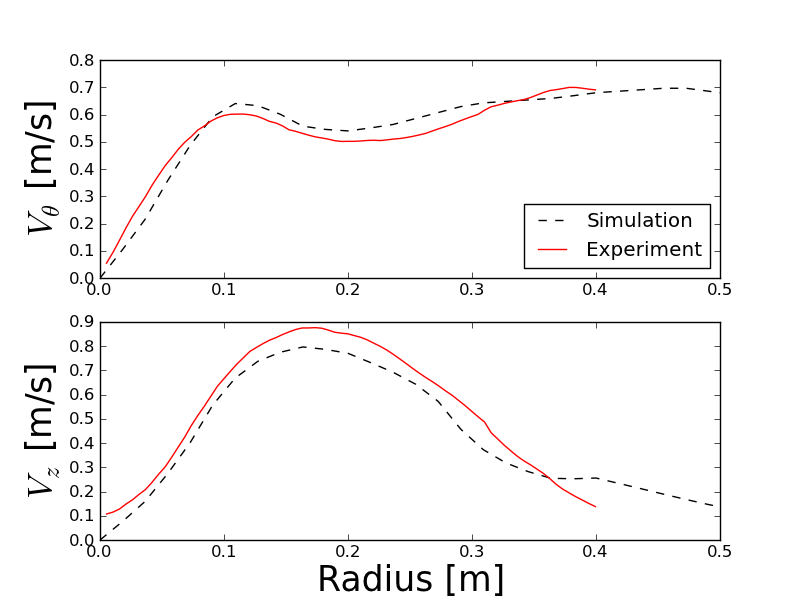
\includegraphics[width = 12 cm]{figs/hybrid_profile}
     \caption{Azimuthal and vertical velocity profiles as a function of
     radius. The simulation and experimental data broadly agree, with
     the simulation also exhibiting the characteristic ``twin-peak''
     structure of the hybrid vanes in the azimuthal velocity. }
     \label{fig:lab}
    \end{center}
  \end{figure}

%
%
%

\subsection{Further Concerns}
%
% no quantitative data from wind cases! 
%
Qualitative agreement between our results and wind tunnel agreement
within 15\% of energy fluxes. Measured in field.\todo{write me!}
%


%
% turbine (explain why we dont need to do it)
%

Another significant validation challenge is in modeling the
turbines. This is in essence a new embedded 
submodel that we will add after validation of the initial configuration
is completed. 
